

ConPaaS is an open-source runtime environment for hosting applications
in Cloud infrastructures~\cite{conpaasIC}.  Within the Cloud computing
paradigm, ConPaaS belongs to the platform-as-a-service family, in
which a variety of systems aim to simplify the deployment of
applications in the Cloud.

%Using ConPaaS,  developers can now focus their attention on application-specific concerns rather than making their applications suitable for the cloud. 

\subsection*{Architecture}

In ConPaaS, an application is designed as a composition of one or more
elastic and distributed \emph{services}. Each service is dedicated to
host a particular type of functionality of an application. ConPaaS
currently supports seven different types of services: two web
application hosting services respectively specialized for hosting PHP
and JSP applications; a MySQL database service; a NoSQL database
service built around the Scalarix key-value store; a MapReduce
service; a TaskFarming service for high-performance batch
processing; and a shared file system service.
%Figure~\ref{arch} shows ConPaaS hosting an application composed of a PhP service and a MySQL service, that could represents the architecture of any today's web application.

Each ConPaaS service is made up of one manager virtual machine (VM)
and a number of agent VMs.

\begin{figure*}[Ht]
\begin{center}
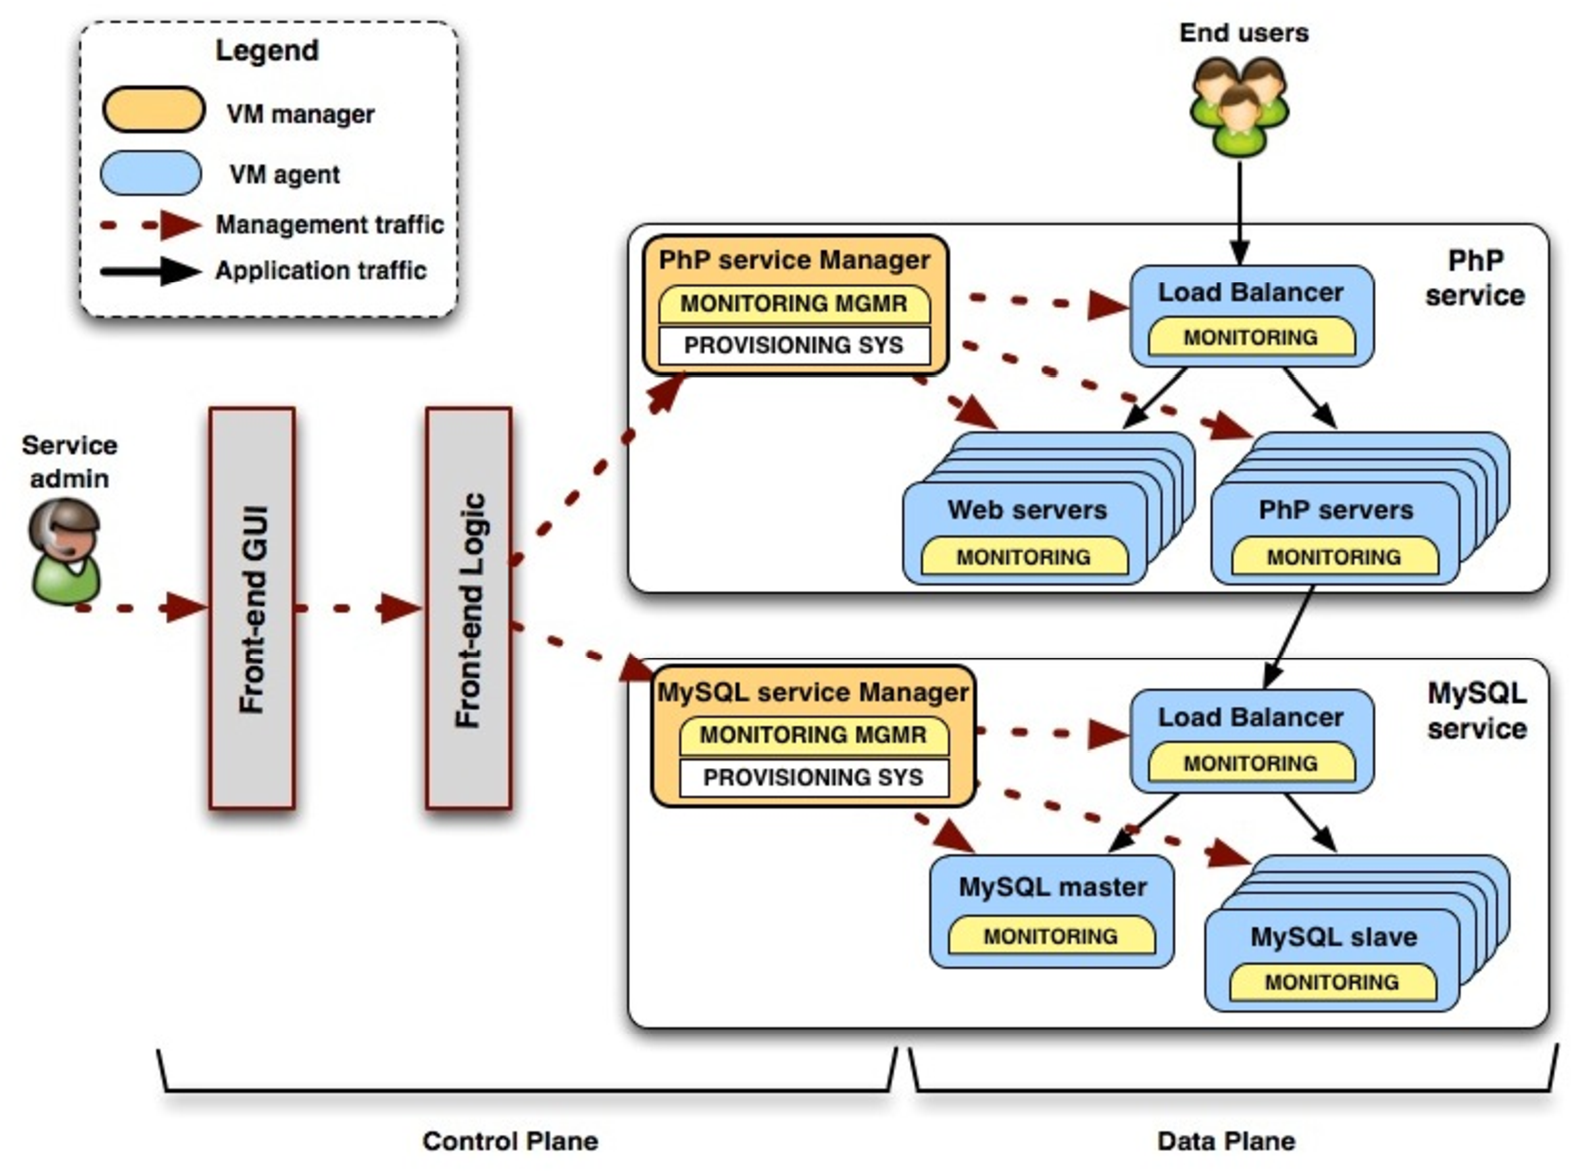
\includegraphics[width=0.6\textwidth, height=6.2cm]{./images/conpaasSystemArch_2}
\end{center}
\vspace{-5mm}
\caption{ConPaaS system architecture.}
\label{arch}
\end{figure*}

\begin{description}
\item[Agent:] The agent VMs host the necessary components to provide the service-specific functionality. Based on the performance requirements or the application workload, agent VMs can be started or stopped on demand. Thus, as an example, the minimal configuration of the PHP web hosting service consists of a single agent VM. If necessary,
the service can grow to multiple agent VMs hosting its
components: load balancer for distributing the incoming traffic, web
servers for static pages and/or PHP servers for dynamic pages.
\item[Manager:] Each service is controlled by one manager VM. The manager is in charge of centralizing monitoring data, controlling the allocation of resources assigned to the service, and coordinating reconfigurations so no loss of service is experienced when adding or removing resources.
\end{description}

Figure~\ref{arch} shows the architecture of the ConPaaS deployment for
a typical PHP web application backed by a MySQL database. The
application is deployed using two ConPaaS services: the PHP service
and the MySQL service.

%On the other hand, in ConPaaS, there are two types of traffic: application and management. The application traffic is based on requests from end users willing to access the application, so that is addressed to the agents hosting such application.  On the other hand, the management traffic is directed from the service administrators to their service managers, and from those to the agents.  Service administrators can manage their services using a graphical front-end or a command-line tool.  

\subsection*{Elasticity}

As illustrated in Figure~\ref{arch}, the manager VM of each ConPaaS
service includes a performance monitoring and a resource provisioning
system.

%ConPaaS incorporates a scalable distributed monitoring engine which is based on the Ganglia~\cite{ganglia} monitoring system. Ganglia consists of a server component (gmetad) that aggregates monitoring statistics from various VMs, and a reporting agent (gmond) which runs inside each VM. By default, Ganglia monitors only system-level metrics such as disk, CPU, memory and network usage. Unfortunately, these metrics often do not provide enough information about system performance due to the heterogeneity of the applications. As a consequence, in ConPaaS, we enhanced ganglia to also monitor service workloads by enhancing the reporting agent to track service-specific logs at runtime, and report statistics over a reporting period of 5 minutes. For instance, the PhP service includes new ganglia metrics that report statistics about the response time and request rate for static and dynamic user requests, respectively. Once the monitoring data is collected from the agents VMs, the resource provisioning  algorithm decides whether to trigger scaling operations based on this data. 

The monitoring component is based on Ganglia~\cite{ganglia}, a
scalable distributed monitoring system. The monitoring data is
collected by the manager VM, which runs a so-called Ganglia
meta-daemon. We implemented modules that extend Ganglia's standard set
of monitoring metrics, by adding a number of service-specific
metrics. In particular for the PHP service, we added monitoring
metrics for measuring the request rate and response times of static
and dynamic documents.

%Unlike of implementing traditional trigger-based provisioning systems that scale services independently of whether they are part of an application. In ConPaaS, we designed a performance control model for multi-service applications. Using this model, the performance requirements are only imposed to the front-end service, while all the services collaborate in order to guarantee them. It improves the effectiveness and accuracy of the scaling decisions. Indeed, this allows to rapidly detect performance bottlenecks in applications, and thereby to minimize the resource consumption.

Each ConPaaS service can plug-in its own automatic resource
provisioning policies, taking into account specificities of the
service such as the structure of the service deployment, the
complexity of the requests and service-specific monitoring data. So
far our focus has been on the web hosting service, for which we
implemented a number of automatic resource provisioning policies.

% Instead of implementing simple performance-based triggers which provision each tier individually based on %its own performance, we designed a performance control model for the entire application. 


%Ganglia stores monitored statistics in a custom roundrobin database (RRD); our monitoring engine can track %resource usage and application workload statistics by periodically querying this database and determining %whether any user-specified thresholds have been exceeded (e.g., thresholds on SLA violations, request %drops, or resource utilization). 

 

